% 课程:人机交互技术及应用
% 班级:传播学1001班
% 课时:40学时,2012年秋季1~10周,每周一、三
% 地点:东九楼D212
% 主页:http://code.google.com/p/hci-course/
% 教师:施展 
% 单位:华中科技大学 武汉光电国家实验室
\documentclass{beamer}
\usepackage{fontspec,xunicode,xltxtra,beamerthemesplit}
%\usetheme{Hannover} % White background
\usetheme{Berkeley} % Blue background
\setsansfont[Mapping=tex-text, ItalicFont={Courier Italic}]{Microsoft YaHei}

% 中文环境自动换行
\XeTeXlinebreaklocale "zh"
\XeTeXlinebreakskip = 0pt plus 1pt

% 中文环境修正导航栏
\makeatletter
\def\beamer@linkspace#1{%
  \begin{pgfpicture}{0pt}{-1.5pt}{#1}{5.5pt}
    \pgfsetfillopacity{0}
    \pgftext[x=0pt,y=-1.5pt]{.}
    \pgftext[x=#1,y=5.5pt]{.}
  \end{pgfpicture}}
\makeatother

\title{人机交互技术}
\author{施展}
\institute{华中科技大学~武汉光电国家实验室}
\date{\today}
\titlegraphic{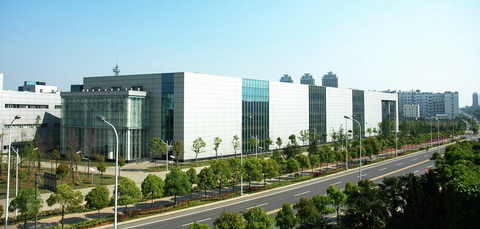
\includegraphics[width=3cm]{images/wnlo.jpg}}

\begin{document}

\begin{frame}
	\titlepage
\end{frame}

\begin{frame}
	\tableofcontents
\end{frame}

\section{课程介绍}
\subsection{教材及参考书}
\begin{frame}
	\frametitle{教材及参考书}
    \transdissolve
	\begin{columns}
		\column{5cm}
			\centerline{\includegraphics[width=2.7cm]<1->{images/textbook.jpg}}\label{textbook}
		\column{5cm}
			\centerline{\includegraphics[width=2.7cm]<2->{images/referencebook.jpg}}\label{referencebook}
	\end{columns}
	\begin{itemize}
		\item<1->[教材] \tiny 孟祥旭,李学庆,杨承磊等:《人机交互基础教程(第2版)》清华大学出版社,2010
		\item<2->[参考] \tiny [美]施奈德曼,[美]普莱萨特,《用户界面设计—有效的人机交互策略(第五版)》,2010
	\end{itemize}
\end{frame}

\subsection{教学目标}
\begin{frame}
	\frametitle{教学目标}
	\begin{itemize}[<+-|alert@+>]
		\item 了解人机交互的含义,人机交互的研究内容及发展趋势;
		\item 了解人机交互的一些新技术,如语音、手写识别、眼动跟踪等技术;
		\item 掌握人机交互的表示模型,并能够进行形式化的描述;
		\item 掌握人机交互界面构造的一般性方法,能够独自设计一个人机交互界面程序;
		\item 了解并掌握认知心理学、人机工程学在人机界面的作用,并在此基础上能够进行人机交互界面给出评价;
		\item 了解Web界面和移动界面设计的流行趋势,掌握Web界面和移动界面设计时需注意的特殊问题。
	\end{itemize}
\end{frame}

\subsection{教学内容}
\begin{frame}
	\frametitle{教学内容}
	\begin{itemize}[<+-|alert@+>]
		\item 人机交互概念
		\item 感知和认知基础
		\item 交互设备
		\item 交互技术
		\item 界面设计 
		\item 人机交互的界面表示模型与实现
		\item Web界面设计
		\item 移动界面设计
		\item 可用性分析与评估
	\end{itemize}
\end{frame}

\subsection{联系我}
\begin{frame}
	\frametitle{联系我}
	\begin{columns}
		\column{5cm}
			\centerline{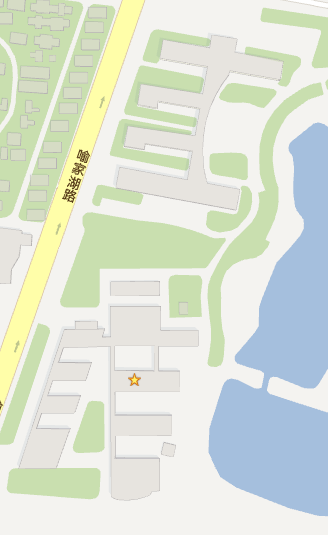
\includegraphics[scale=0.3]{images/maps.google.com_2012-9-2_11_6_22.png}}\label{WNLO_location_map}
		\column{5cm}
			\centerline{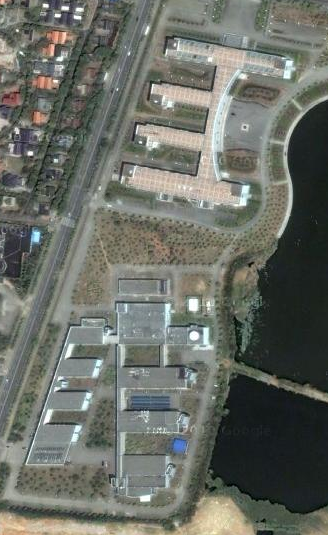
\includegraphics[scale=0.3]{images/maps.google.com_2012-9-2_11_7_11.png}}\label{WNLO_location_sat}
	\end{columns}
	\begin{itemize}
		\item \small{工作地点:武汉光电国家实验室 F座309}
		\item \small{电话:13971459597}
		\item \small{课程网站:\textit{http://code.google.com/p/hci-course/}}
	\end{itemize}
\end{frame}

\section{第一章}
 
\begin{frame}
	\frametitle{第一章}
	\begin{itemize}[<+-|alert@+>]
		\item have 1
		\item have 2
		\item have 4
		\item .......
	\end{itemize}
\end{frame}
 
\section{本章小节}
\begin{frame}
	\frametitle{本章小节}
	sth...
	\begin{itemize}[<+-|alert@+>]
		\item 1
		\item 2
	\end{itemize} 
	\hfill \\
	else ?...
\end{frame}
 
\end{document}